\documentclass[tikz,border=0pt]{standalone}
\usepackage[american]{circuitikz}
\usetikzlibrary{arrows.meta,calc,positioning,decorations.pathmorphing,patterns}
\definecolor{zyloTeal}{HTML}{174A5B}
\definecolor{zyloTealTwo}{HTML}{246B7A}
\definecolor{zyloInk}{HTML}{1F2933}
\definecolor{zyloSoft}{HTML}{EAF4F4}
\definecolor{zyloPaper}{HTML}{F8FAFB}
\definecolor{zyloLine}{HTML}{44606B}
\definecolor{zyloOrange}{HTML}{D97706}
\begin{document}
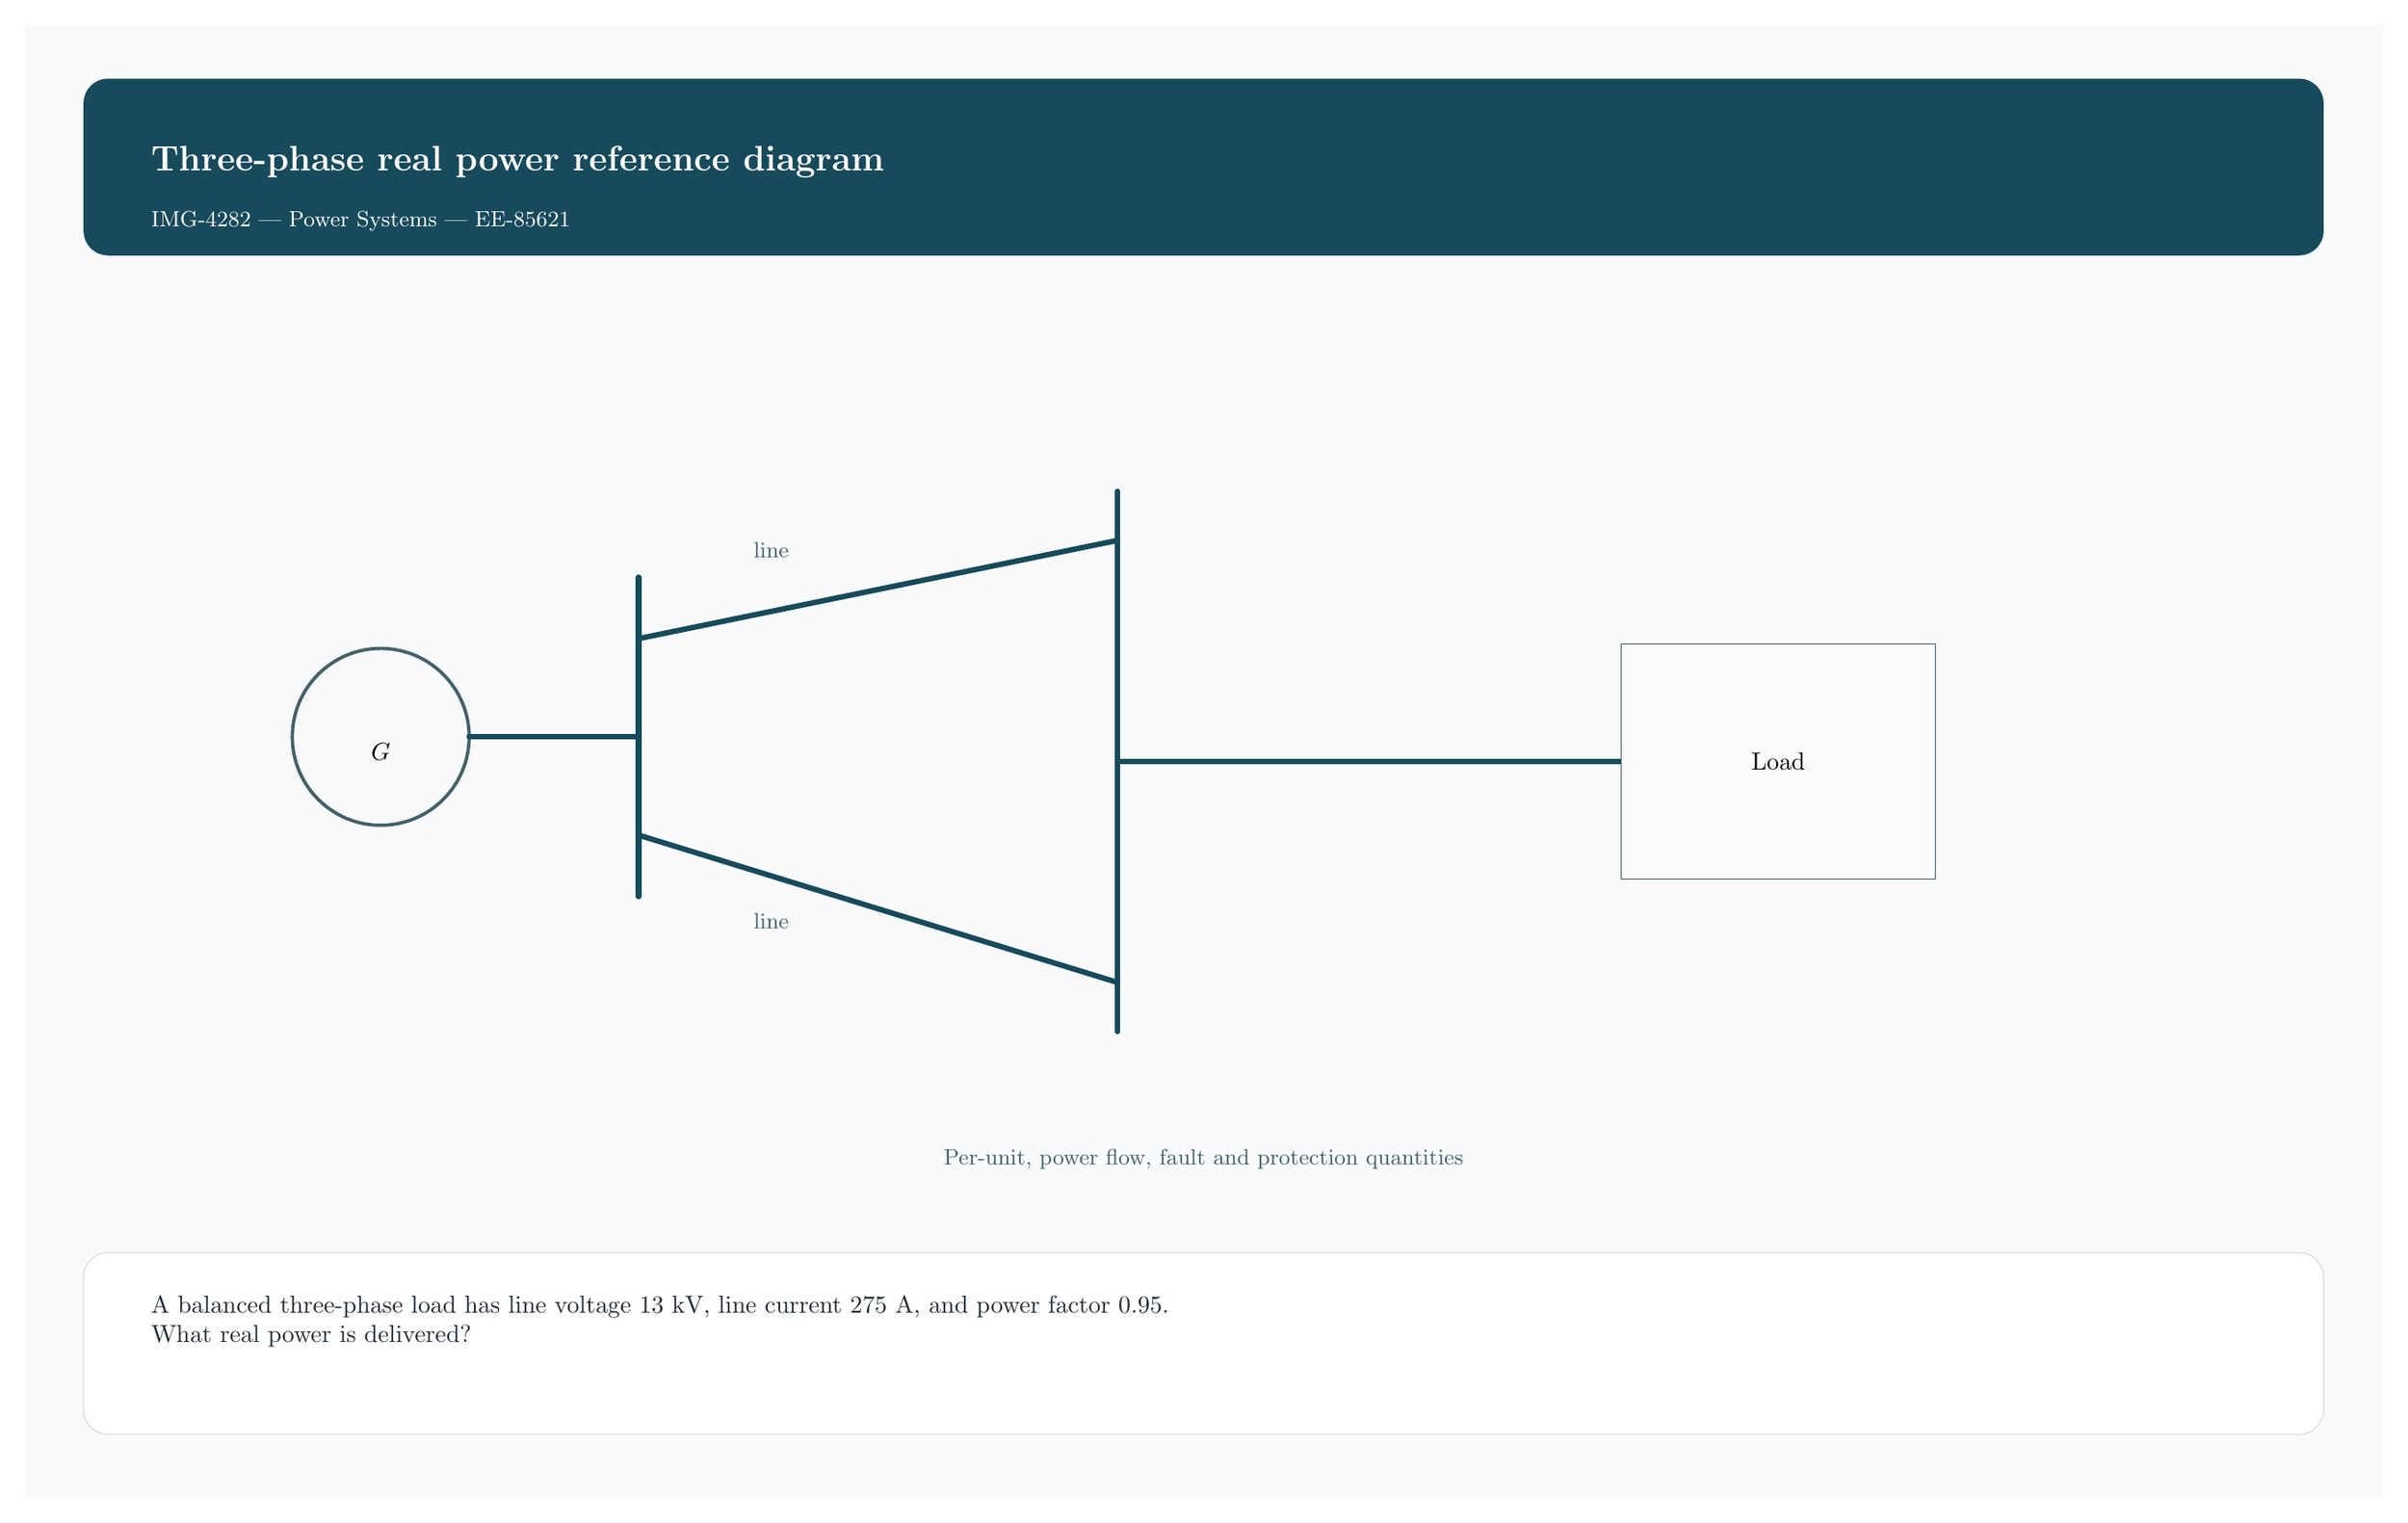
\begin{tikzpicture}[x=1pt,y=-1pt,>=Latex,line cap=round,line join=round]
\path[fill=zyloPaper] (0,0) rectangle (960,600);
\path[fill=zyloTeal,rounded corners=10pt] (24,22) rectangle (936,94);
\node[anchor=west,text=white,font=\bfseries\Large] at (48,56) {Three-phase real power reference diagram};
\node[anchor=west,text=white!82,font=\small] at (48,80) {IMG-4282 | Power Systems | EE-85621};
\tikzset{wire/.style={draw=zyloTeal,line width=2.2pt},thinwire/.style={draw=zyloLine,line width=1.35pt},accent/.style={draw=zyloOrange,line width=2.2pt},box/.style={draw=zyloTealTwo,fill=zyloSoft,line width=1.5pt,rounded corners=8pt}}
\draw[thinwire] (145,290) circle (36); \node at (145,296) {$G$};
\draw[wire] (181,290) -- (250,290);
\draw[wire] (250,225) -- (250,355);
\draw[wire] (250,250) -- (445,210);
\draw[wire] (250,330) -- (445,390);
\draw[wire] (445,190) -- (445,410);
\draw[wire] (445,300) -- (650,300);
\node[draw=zyloLine,fill=white!80!zyloSoft,minimum width=128pt,minimum height=96pt] at (714,300) {Load};
\node[font=\small,text=zyloLine] at (304,214) {line}; \node[font=\small,text=zyloLine] at (304,365) {line};
\node[font=\small,text=zyloLine] at (480,462) {Per-unit, power flow, fault and protection quantities};
\path[draw=black!15,fill=white,rounded corners=10pt] (24,500) rectangle (936,574);
\node[anchor=west,text width=860pt,align=left,text=zyloInk,font=\normalsize] at (48,528) {A balanced three-phase load has line voltage 13 kV, line current 275 A, and power factor 0.95.\\What real power is delivered?};
\end{tikzpicture}
\end{document}
